\documentclass[conference,compsoc]{IEEEtran}

\usepackage{cite}
\usepackage{amsmath,amssymb,amsfonts}
\usepackage{algorithmic}
\usepackage{graphicx}
\usepackage{textcomp}
\usepackage{xcolor}
\def\BibTeX{{\rm B\kern-.05em{\sc i\kern-.025em b}\kern-.08em
    T\kern-.1667em\lower.7ex\hbox{E}\kern-.125emX}}
    
\usepackage{epigraph}
\usepackage{listings}
\usepackage{adjustbox}
\usepackage{multirow}
\usepackage{array}
\usepackage{authblk}

\usepackage[hyphens]{url}

\newcommand{\myparagraph}[1]{\smallskip\noindent{\bf #1.}}
\newcommand{\myfirstparagraph}[1]{\noindent{\bf #1.}}
\newcommand{\scedit}[1]{{\color{black} #1}} % blue
    
\begin{document}

\title{FuzzSplore: Visualizing Feedback-Driven Fuzzing Techniques}

\iffalse
\author{\IEEEauthorblockN{Andrea Fioraldi}
\IEEEauthorblockA{\textit{1692419}}
\and
\IEEEauthorblockN{Luigi Paolo Pileggi}
\IEEEauthorblockA{\textit{0000000}}
}

\author{\IEEEauthorblockN{Andrea Fioraldi\IEEEauthorrefmark{1}\IEEEauthorrefmark{2},
Luigi Paolo Pileggi\IEEEauthorrefmark{1}}
\IEEEauthorblockA{andreafioraldi@gmail.com,
gigimail@gigi.com\\
\IEEEauthorrefmark{1} Sapienza University of Rome,
\IEEEauthorrefmark{2} EURECOM}}
\fi

\author[1,2]{Andrea Fioraldi}
\author[1]{Luigi Paolo Pileggi}
\affil[1]{Sapienza University, Rome, Italy \authorcr {\tt \{fioraldi.1692419, pileggi.0000000\}@studenti.uniroma1.it}\vspace{1.5ex}}
\affil[2]{EURECOM, Sophia Antipolis, France \authorcr {\tt fioraldi@eurecom.fr} \vspace{-2ex}} 

\maketitle

\section{Introduction}

{\it Feedback-driven Fuzz Testing} is a family of techniques to automatically uncovers bugs in software.

Due to its effectiveness, much more efficient than other software testing techniques like {\it Symbolic Execution} \cite{redqueen} \cite{sebastian}, the research in this field is flourishing and several different techniques were developed to improve fuzz testing, both from academy and industry.

The evaluation and the comparison of these techniques, however, is a debatable matter \cite{fuzzeval}.

A common proxy is the comparison of the code coverage reached over time by each fuzzer, due to the fact that a fuzzer cannot find a bug if it does not explore at least the vulnerable code segment.
Another widely used metric is found bugs over time, but a bug can be found just thanks to randomism and this makes the evaluations very prone to overfitting.

The data collected using these metrics are often representable using a simple time-based graph that shows the evolution of the fuzzing algorithm.

This approach is useful for an immediate basic comparison between two or more techniques, an analyst have to just see which technique reaches more coverage in less time, but does not reveal the properties of a fuzzer regards specific types of programs states.

For instance, a technique can be better than another in exploring some types of program states and in the same time reaching less code coverage.
The technique will not cover the bugs in the unexplored code of course, but it may uncover bugs in the program points that it can better explore.
An example of such technique is the directed fuzzer towards sanitizers violations by \"Osterlund et al. \cite{parmesan}.

We propose {\sc FuzzSplore}, a tool that allows an analyst to manually explore the evolution of different fuzzing techniques on the same target program.

The main insight that an user can get using the tool are:

\begin{enumerate}
\item The ability of a fuzzer to generate clusters of inputs that are correlated in terms of covered program points;
\item The ability of a fuzzer in generating diversified inputs with its mutational algorithm;
\item The ability of a fuzzer to reach program points exploring intermediate inputs that are not an improvement in terms of coverage \cite{besensitive}.
\end{enumerate}

These insights can drive the user in the choice of the best technique to use for the selected program under test (PUT).

\section{Background}

The simplest description of Feedback-driven Fuzzing is an algorithm that provides apparently random data to a computer program and then it watches for crashes or unexpected states and also saves the generated input for later processing if they covers interesting new states that are used as feedback \cite{fuzzing-book}.

Tipically, the program states used as feedback are the edges in the program Control Flow Graph \cite{compilerbook} in what is the so-called {\it Coverage-guided Fuzzing} (CGF).

The inputs are mutations of previously saved inputs in the fuzzing loop in Mutational Fuzzing or generated from scratch from a model in Generational Fuzzing.

Our baseline, {\sc AFL++} \cite{aflplusplus}, a widely used fuzzer in the recent times, is a Mutational Coverage Guided Fuzzer.

\begin{center}
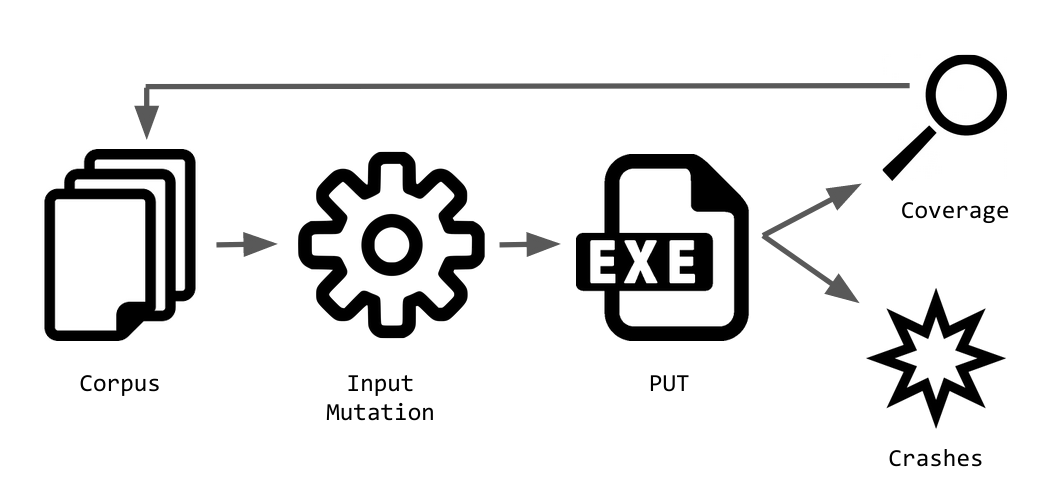
\includegraphics[scale=0.16]{cgf}
\end{center}

State of the art Coverage-Guided Fuzzers encode the approximate executed path in a representation that is easy and fast to process.
{\sc AFL++} uses a vector of 65536 entries, the {\it hitcounts} vector.

Each coordinate is associated with an edge and each value represents how many times the edge is executed modulo 256.

When a values greater than the previous one is registered in this vector, the fuzzer consider the input interesting and saves it.

Some extensions of CGF save also intermediate inputs that are a superset of the coverage reported in the hitcounts vector, like \cite{lafintel} \cite{ijon} \cite{besensitive}.

In general, when an input is saved, we can associate it to the testcase that generated it by mutation, the {\it parent} testcase. In this way, is easy to construct a tree of generated inputs that represents the progress of the hill climbing algorithm of the fuzzer, the {\it levels} tree.

Looking for parents in this tree, we can evaluate if the intermediate inputs generated by the specific technique is effective.

\section{Proposal}

We propose a time-based visualization of the progress of different techniques based on {\sc AFL++}.

The first view will be a navigable levels tree. The user can select the technique in a scrollbar and view the associated tree.

Each node of the tree can be selected to view if it can be considered an interesting input for another technique. This will help in understanding the insight 3, were a tecnhique rech a program points thanks to an intermediate input that another technqiue cannot see as interesting.

There will be also a scatterplot representing the inputs in terms of covered state.
We collect the hitcounts vector of each input, reduce the dimensionality using PCA and then apply t-SNE on the vector with reduced dimensions to preserve outliners in these most important dimensions.

The color of each point will be related to the technique that generated the input.

In this scatterplot, the user can manually select a cluster of points that represents inputs with related paths.

Of course it can choose to consider only a subset of the techniques and hide that points from the view.

Doing that, will help to cope the insight number 1 looking at the density of the cluster for each different technique.

When doing this, the user can then choose to highlight in the scatterplot the inputs that are parents for the points in the cluster.

A technque that is able to generate inputs from other that are almost completely unrelated have a better mutational algorithm than a technqiue that generate inputs similar to the parents, this helps the analyst with insight number 2.

The tree an the scatterplot are synchronized. When a cluster is selected, the corresponding inputs are highlighted in the tree.

All these points can be hidden using a time bar. Selecting a specific lapse of time, only inputs founds by the fuzzer before that time are considered.

The other two views, related to the evolution in time, are the coverage over time graph and the new interesting inputs per seconds graph.

When a testcase is selected (both in the scatterplot or in the tree) a line appears in these graphs highlighing the time in which the testcase was discovered.

Coverage over time shows when an input that is important in terms of new coverage is found and so suggest the user where it should put the time bar for a targeted analysis.

Inputs per seconds is related with the levels tree. If a fuzzer generates too many intermediate testcases it can saturate the evolution of the alogrithm, so if we select an intermediate input in the levels tree and see an peak in this graph likely the technique suffers from path explosion.

\begin{center}
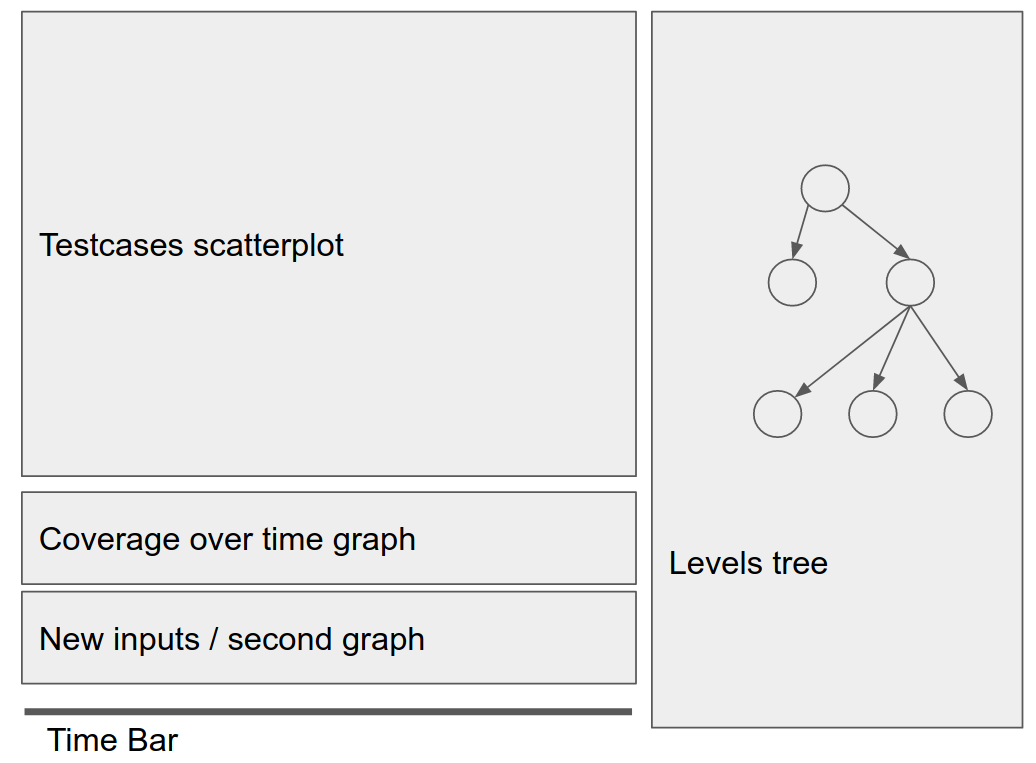
\includegraphics[scale=0.2]{mockup}
\end{center}

\bibliographystyle{IEEEtran}
\bibliography{bibliography}

\end{document}
